%%%%%%%%%%%%%%%%%%%%%%
% Does Presidential Partisanship Affect Fed Inflation Forecasts?
% Christopher Gandrud & Cassandra Grafström
% Updated 28 October 2012
%%%%%%%%%%%%%%%%%%%%%%

\documentclass{beamer}
\usetheme{MichiganYonsei}
\setbeamercovered{transparent}
\usepackage{color}
\usepackage{hyperref}
  \hypersetup{
		colorlinks=true
		linkcolor=black
		}
\usepackage{graphics}
\usepackage{booktabs}
\usepackage{url}
\newcommand{\comment}[1]{}


%%%%%%%%%%%%%%%%%%%%%%%%%%%%%%%% Title Slide %%%%%%%%%%%%%%%%%%%%%%%%%%
\title[Partisan Inflation Forecast Errors]{Does Presidential Partisanship Affect Fed Inflation Forecasts?}
\author[]{
    \href{mailto:gandrud@yonsei.ac.kr}{Christopher Gandrud} \and         \href{mailto:{cgrafstr@umich.edu}}{ Cassandra Grafstr\"{o}m}
}


\begin{document}

\frame{\titlepage}

\section[Outline]{}
\frame{\tableofcontents}

%%%%%%%%%%%%%%%%%%%%%%%%%%%%%%%%% Motivation %%%%%%%%%%%%%%%%%%%%%%%%%%%%%%%%%%%%%
\section{Motivation}
\frame{
  \frametitle{Working Paper}
  \begin{center}
    {\Large{The working paper is available on SSRN at: \\[0.5cm] \url{http://papers.ssrn.com/sol3/papers.cfm?abstract_id=2105301}.}}
  \end{center}
}

\frame{
  \frametitle{Presidential Partisan Inflation Forecast Bias}
  {\Large{Presidential Partisan Inflation Forecast Bias:}}\\[0.5cm] 
  When inflation forecasts are systematically different depending on the partisan identification of the United States president.
}

\frame{
    \frametitle{Motivation}
    {\LARGE{Why should we care about presidential partisan inflation forecast bias?}} \\[0.5cm]
        \begin{itemize}
            \item<1-> Clark \& Arel-Bundock (2011) find policymakers at the Federal Reserve are not politically indifferent.
            \item<2-> Could be that the information they receive is biased.
		\item<3-> Economists have not considered political preferences when evaluating Fed accuracy.
        \end{itemize}
}     

%%%%%%%%%%%%%%%%%%%%%%%%%%%%%%%%% Describing Forecast Errors %%%%%%%%%%%%%%%%%%%%%%%%%%%%%%%%%%%%%

\section{Describing Forecast Errors}
\frame{
    \frametitle{Forecast Accuracy}
        \begin{center}
            {\LARGE{How accurate are Fed inflation forecasts?}}
        \end{center}
}

\frame[plain]{
    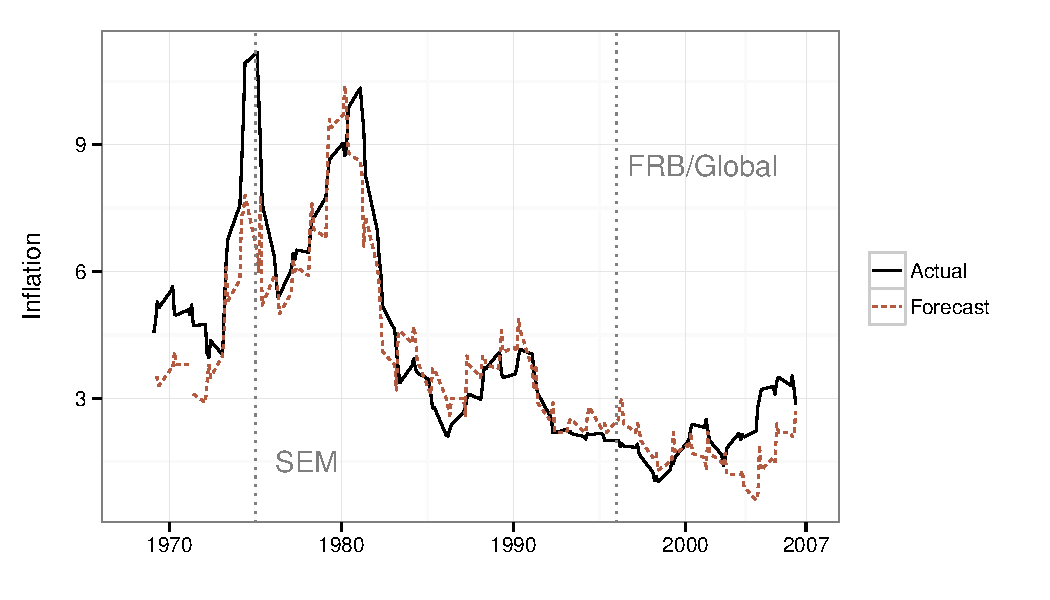
\includegraphics[scale=0.65]{/git_repositories/GreenBook/Paper/figure/BaseInflation.pdf}
}

\frame{
  \frametitle{Forecast Errors}
  Our {\bf{dependent variable}}: \\[0.5cm]
\[
    E_{q} = \frac{F_{q} - I_{q}}{I_{q}}
\]
  \begin{itemize}
    \item<2-> $E_{q} = $ the standardized inflation forecast error for quarter $q$.
    \item<3-> $F_{q} = $ Green Book inflation forecast for quarter $q$. (We use forecasts made {\emph{two quarters}} prior).
    \item<4-> $I_{q} = $ actual inflation in quarter $q$.
  \end{itemize}
}

\frame{
  \frametitle{Forecast Errors}
  \begin{center}
    {\LARGE{Ideally, the mean forecast error is 0.}} \\[0.5cm]

	{\large{Consistent errors $\rightarrow$ ``wrong" policies.}}
  \end{center}
}

\frame[plain]{
  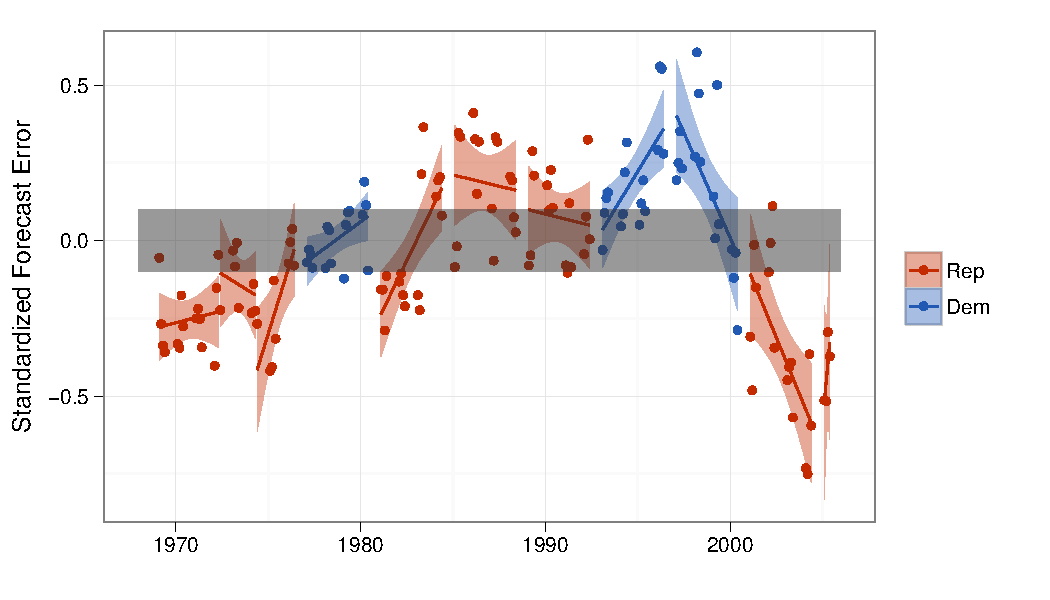
\includegraphics[scale=0.65]{/git_repositories/GreenBook/Paper/figure/partisanError.pdf}
}

%%%%%%%%%%%%%%%%%%%%%%%%%% What might explain forecast errors? %%%%%%%%%%%%%%%%%%%%%%%%%%%%%%%

\section{What Might Explain Forecast Errors?}
\frame{
    \frametitle{Possible explanations}
        \begin{center}
            {\LARGE{What might explain forecast errors?}}
        \end{center}
}

\frame{
  \frametitle{Traditional understanding of Fed forecasting}
\begin{itemize}
	\item<1-> Forecasts produced for every FOMC meeting
	\item<2-> Over long run no bias (e.g., Romer and Romer 2000).
	\item<3-> Periods of over- and under-estimations (Capistr\'{a}n 2008).
	\item<4-> No research on partisan influence of forecast errors.
\end{itemize}
}

\frame[plain]{
  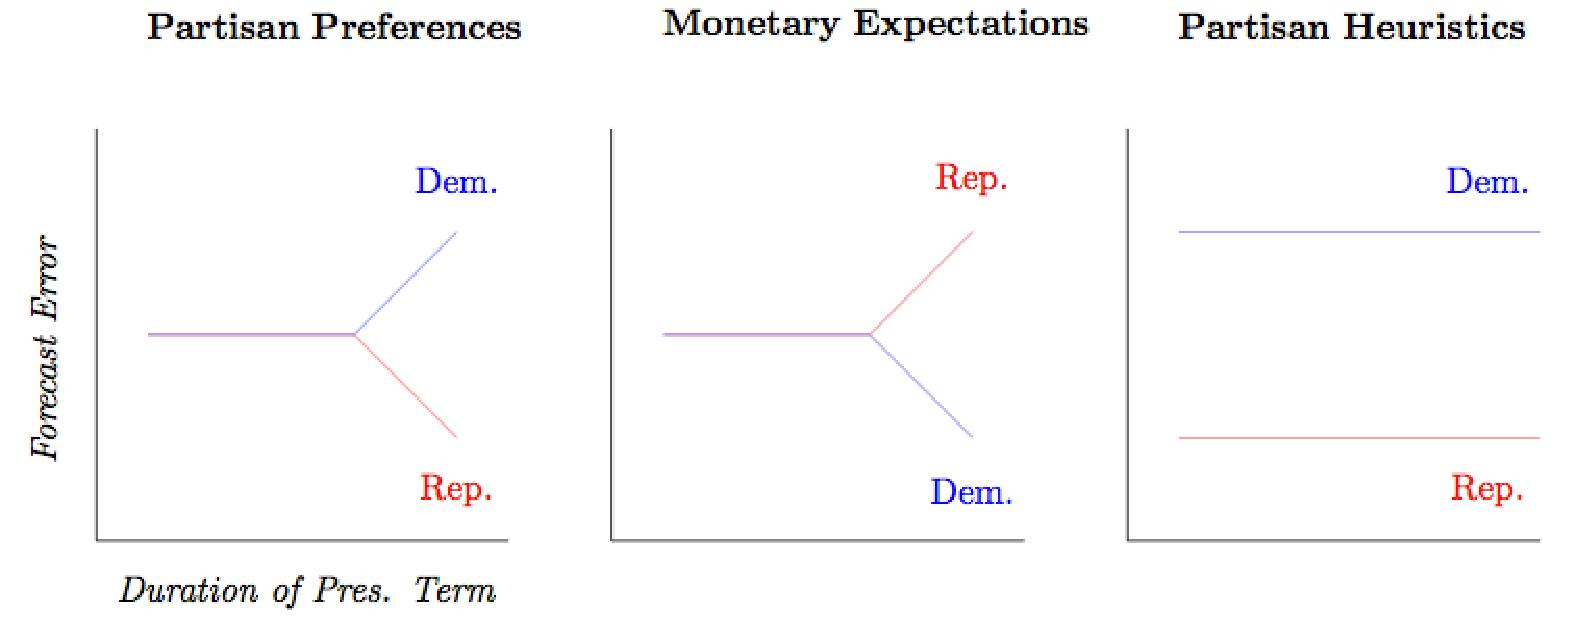
\includegraphics[scale=0.4]{ExpectationsGraph.pdf}
}

%%%%%%%%%%%%%%%%%%%%%%%%%% Empirical Tests %%%%%%%%%%%%%%%%%%%%%%%%%%%%%%%


\section{Empirical Tests}
\frame{
  \frametitle{Empirical Analysis Overview}
    \begin{center}
      {\LARGE{Followed Ho et al. (2010) to isolate relationship between presidential partisanship/elections and the other controls.}} \\[0.5cm]
    \end{center}
    \begin{enumerate}
      \item<2-> Two data sets {\bf{matched}} on:
        \begin{itemize}
            \item<2-> {\emph{presidential party ID}}
            \item<2-> {\emph{election period}}
        \end{itemize}
      \item<3-> Used these in {\bf{parametric models}} with standardized inflation forecast errors as continuous dependent variable. 
    \end{enumerate}
}

\frame{
    \frametitle{}
        \begin{center}
            {\LARGE{Results?}}
        \end{center}
}

\frame[plain]{
  \begin{center}
    {\LARGE{Main Results}} (2 Quarter Old Forecasts)
  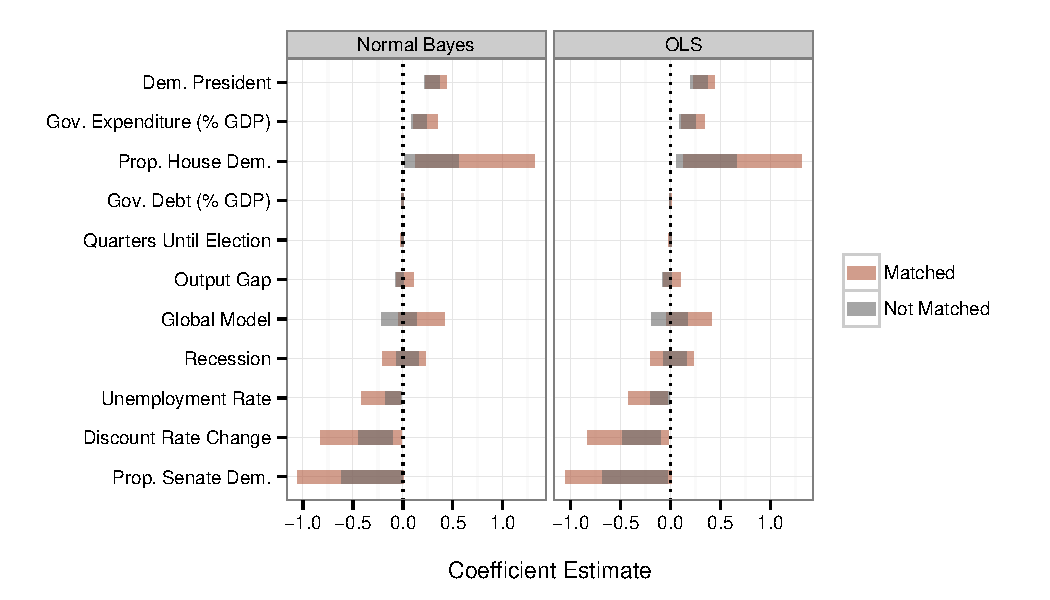
\includegraphics[scale=0.65]{/git_repositories/GreenBook/Paper/figure/CoefComparePlots.pdf}
  \end{center}
}

\frame[plain]{
  \begin{center}
    {\LARGE{Simulated Errors}} (All Forecasts)
    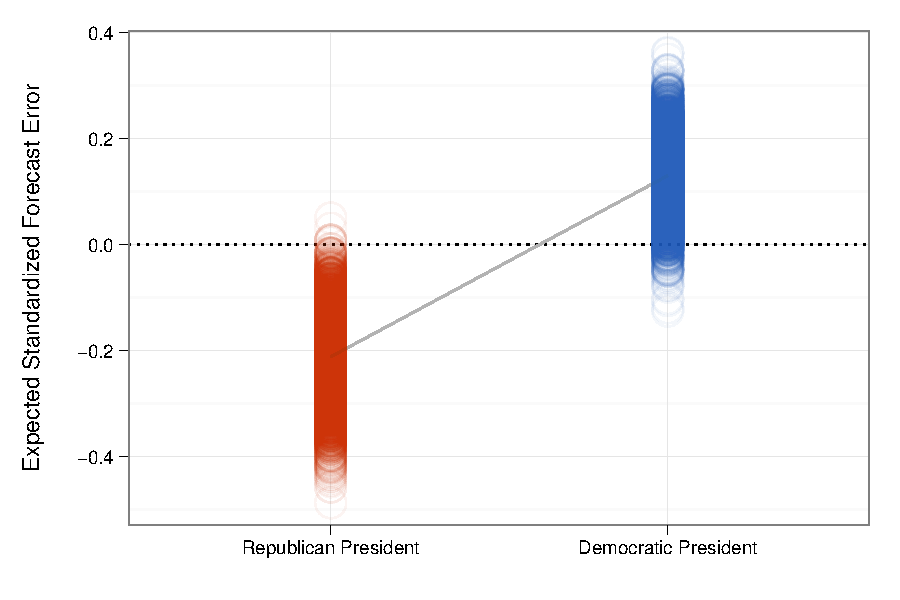
\includegraphics[scale=0.65]{/git_repositories/GreenBook/Paper/figure/ExpectValueParty.pdf}
  \end{center}
}

\frame[plain]{
  \begin{center}
    {\LARGE{Interactions}} (2 Quarter Old Forecasts)
  \end{center}
  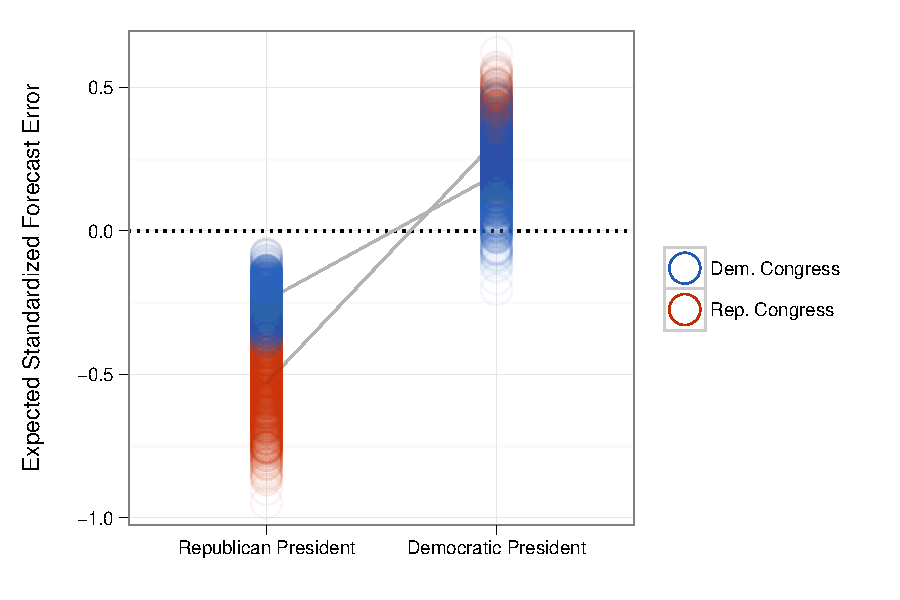
\includegraphics[scale=0.65]{/git_repositories/GreenBook/Paper/figure/InterPlot.pdf}
}

%%%%%%%%%%%%%%%%%%%%%%%%%% Conclusions %%%%%%%%%%%%%%%%%%%%%%%%%%%%%%%

\section{Conclusions}
\frame{
    \frametitle{Conclusions}
    {\LARGE{Does presidential partisanship affect Fed staff inflation forecasts? \\[1cm]
        \begin{center}
            Probably.
        \end{center}
        }
    }
}

\frame{
  \frametitle{Conclusions}
  {\LARGE{How?}} \\[0.5cm]
  \begin{itemize}
    \item<1-> Fed staff {\bf{don't}} have an electoral bias. 
        \begin{itemize}
            \item<2-> Don't seem to try to influence election outcomes or compensate for FOMC political preferences.
        \end{itemize}
         \\[0.3cm]
    \item<3-> Fed staff {\bf{do}} use a {\bf{partisan heuristic}} 
		\begin{itemize}
			\item Leads to {\bf{systematic bias}} in inflation forecasts across presidential terms.
		\end{itemize}
  \end{itemize}
}

\frame{
  \frametitle{Conclusions}
  {\LARGE{Possible political implications?}} \\[0.5cm]
  \begin{itemize}
    \item<1-> High inflation forecasts during {\bf{Democratic}} presidencies $\rightarrow$ interest rates {\bf{`too high'}}. 
	\begin{itemize}
		\item This could hurt Democrats' re-election chances.
	\end{itemize}
    \item<2-> Low forecasts during {\bf{Republican}} presidencies $\rightarrow$ interest rates {\bf{`too low'}}. 
	\begin{itemize}
		\item This could help Republicans' re-election chances.
	\end{itemize}
 \\[0.3cm]
	\item<3-> Does not explain Clark and Arel-Boondock's interest rate finding.
    \item<4-> Of course, {\bf{more research is needed}}.
  \end{itemize}
}



\end{document}